\documentclass{article}
\usepackage[utf8]{inputenc}
\usepackage{graphicx}
\graphicspath{ {images/} }
\usepackage{multicol}
\setlength{\columnsep}{2cm}

\documentclass[a4paper]{article}
\usepackage[cp1251]{inputenc}
\usepackage[russian]{babel}
\begin{document}

\begin{titlepage}
	\centering
	{\scshape\LARGE Московский физико-технический институт \par}
	\vspace{3cm}
	{\scshape\Large Лабораторная работа \par}
	\vspace{1cm}
	{\huge\bfseries Исследование взаимной диффузии газов \par}
	\vspace{1cm}
	%{\Large\itshape John Birdwatch\par}
	\vfill
\begin{flushright}
	{\large выполнила студентка 653 группы ФФКЭ}\par
	\vspace{0.3cm}
	{\LARGE Карпова Татьяна}
\end{flushright}
	

	\vfill

% Bottom of the page
	Долгопрудный, 2017 г.
\end{titlepage}

\section{Цель работы}
\begin{enumerate}
    \item Регистрация зависимости концентрации гелия в воздухе от времени с помощью датчиков теплопроводности при разных начальных давлениях смеси газов
    \item Определение коэффициента диффузии по результатам измерений
\end{enumerate}

\section{В работе используются}
\begin{itemize}
    \item измерительная установка
    \item форвакуумный насос
    \item баллон с газом (гелий)
    \item манометр
    \item источник питания
    \item магазин сопротивлений
    \item гальванометр
    \item программа по дополнительнуому описанию эксперимента
\end{itemize}

\section{Теоретические положения}
\begin{enumerate}
\item {\sl Диффузия} - самопроизвольное взаимное проникновение веществ друг в друга, происходящее вследствие хаотичного теплового движения молекул. При перемешивании молекул разного сорта говорят о {\sl взаимной} (или {\sl концентрационной}) диффузии.
В системе, состоящей из двух компонентов, плотность потока вещества в результате взаимной диффузии описывается законом Фика:
\begin{center}
$j_a = -D_a_b\frac{\partial n_a}{\partial x}$, $j_b = -D_b_a\frac{\partial n_b}{\partial x}$,
\end{center}
где $D_a_b = D_b_a = D$ - {\sl коэффициент взаимной диффузии} компонентов, $j_a_,_b$ = плотности потока частиц соответствующего сорта (количество частиц, пересекающих единичную площадку в единицу времени).\\
В работе исследуется диффузия примеси лёгкого газа (гелия) на фоне воздуха, поэтому концентрация воздуха в опыте значительно больше концентрации гелия, и её относительное изменение незначительно. В процессе работы будет описываться только диффузия примеси гелия на стационарном фоне воздуха.\\

\item Проведём теоретическую оценку величины коэффициента взаимной диффузии. В работа мала концентрация гелия, более того, масса атомов гелия много меньше массы молекул, составляющих воздух. При таких условиях перемешивание газов в эксперимента можно рассматривать как диффузию гелия на стационарном форне воздуха. Тогда коэффициент диффузии приблизительно равен
\begin{center}
$D = \frac{1}{3}\lambda \bar v$,
\end{center}
где $\lambda$ - длина свободного пробега частиц гелия, $\bar v = \sqrt{\frac{8kT}{\pi m}}$ - их средняя тепловая скорость. В общем случае необходимо считать $\lambda = \frac{1}{n_\Sigma \sigma}$, где $n_\Sigma = n_H_e + n_B = \frac{P_\Sigma}{kT}$ - полная концентрация частиц, $\sigma$ -  среднее сечение столкновения частиц гелия с воздухом. Также  $\bar v = \sqrt{\frac{8kT}{\pi \mu}}$ - средняя относитель. Таким образом, теоретическая оценка предполагает, что коэффициент диффузии не зависит от пропорция элементов, а обратно пропорционален давлению $D \propto \frac{1}{P_\Sigma}$.
\item  Рассмотрим процесс выравнивания концентрации в установке, она зависит от координат и времени во всей установке. Объём соединительной трубки мал по сравнению с с объёмами сосудов. Поэтому концентрации газов можно считать постоянной по всему объёму сосудов; считаем, что процесс выравнивания происходит только за счёт диффузии в трубке и является стационарным (так как считаем стационарным поток частиц). Величина этого стационарного потока $J = -DS\frac{\partial n}{\partial x}$, и он одинаковый во всём сечении трубки, тогда $n(x)$ - линейная функция координаты и $\frac{dn}{dx} = \frac{\triangle n}{l}$ (l - длина трубки), получаем 
\begin{center}
$J = -DS \frac{n_1-n_2}{l}$.
\end{center}
Предположим, что установился линейный профиль концентрации и полученное соотношение справедливо в любой момент времени. Получаем {\sl квазистационарное} приближение зависимости концентраций $n_1$ и $n_2$ от времени.
\item Через $\triangle n_1$ и $\triangle n_2$ обозначим изменения концентрации в объёмах $V_1$ и $V_1$ за время $\triangle t$. Тогда $V_1 \triangle n_1$ - изменение количества компонента в объёме $V_1$, а $V_2 \triangle n_2$ - изменение количества этого компонента в объёме $V_2$. По закону сохранения вещества следует, что $V_1 \triangle n_1 + V_2 \triangle n_2 = const$, поэтому $V_1 \triangle n_1 = - V_2 \triangle n_2$. Эти изменения происходят вследствие диффузии, поэтому 
\begin{center}
$V_1 \triangle n_1 = - V_2 \triangle n_2 = J \triangle t = -DS \frac{n_1-n_2}{l} \triangle t$
\end{center}
Делим равенство на $\triangle t$
\begin{center}
$V_1 \frac{dn_1}{dt} = -DS\frac{n_1-n_2}{l}$, $V_2 \frac{dn_2}{dt} = -DS\frac{n_1-n_2}{l}$
\end{center}
Делим первое уравнение на $V_1$, второе на $V_2$, вычтем равенства друг из друга:
\begin{center}
$\frac{dn_1}{dt}- \frac{dn_2}{dt} = - \frac{n_1-n_2}{l}DS(\frac{1}{V_1} +\frac{1}{V_2} )$.
\end{center}
Введём новую переменную $\triangle n = n_1-n_2$, проинтегрируем уравнение, получим
\begin{center}
$\triangle n = \triangle n_0 e^(^-^t^/^\tau^)$,
\end{center}
где $\triangle n_0$ - разность концентраций примеси в начльный момент времени, а
\begin{center}
$\tau = \frac{V_1 V_2}{V_1 + V_2} \frac {l}{SD}$.
\end{center}
Видим, что разность концентраций убывает по экспоненциальному закону и тем быстрее, чем меньше $\tau$ - величина, определяющаяся геометрическими параметрами установки и величиной коэффициента диффузии.
\item Для проверки применимости квазистационарного течения убедимся, что время $\tau$ много больше характерного времени диффузии одной частицы вдоль трубки длиной l: $t_d_i_f_f \sim \frac{l^2}{D} \ll \tau$.

\item Для измерения концентраций применяются датчики теплопроводности $D_1$ и $D_2$ (см. рис. 1) и используется зависимость теплопроводности газовой смеси от её состава. Тонкая проволока радиуса $r$, протянутая вдоль оси цилиндра радиуса $R$, нагревается током. Тепло от проволоки к стенке цилиндра передаётся главным образом вспледствие теплороводности газа, находящегося внутри цилиндра. Количество тепла переданного стенке цилиндра в единицу времени, определяется по формуле 
\begin{center}
$Q = \kappa \frac{2\pi L}{ln (R/r)}(T_1-T_2)$,
\end{center}
где $\kappa$ - теплопроводность, $L$ - длина нити, $T_1, T_2$ - температуры проволочки и стенки. При $Q = const$ температура проволоки и её сопротивление определяются теплопроводностью газа и, следовательно, его составом. Для измерения разности концентраций газов используется  
мостовая схема, представленная на рис. 2 (см. пункт 4).

\item В процессе диффузии разность концентраций убывает по экспоненциальному закону. По тому же закону изменяются во времени показания гальванометра:
\begin{center}
$U = U_0 e^(^-^t^/^\tau^)$
\end{center}
Измеряя экспериментально зависимость $U(t)$, можно получить характерное время процесса $\tau$, откуда определить коэффициент диффузии D.
\end{enumerate}

\section{Экспериментальная установка}

\begin{enumerate}
\item Общий вид конструкции установки приведён на рис. 1. Установка состоит из двух сосудов $V_1$ и $V_2$, соединённых краном $K_3$, форвакуумного насоса Ф.Н. с выключателем Т, манометра М и системы напуска гелия, состоящей из кранов $K_6, K'_6, K_7$. Кран $K_5$ позволяет соединять форвакуумны насос либо с установкой, либо с атмосферой. Сосуды $V_1$ и $V_2$ соединены трубкой длины $l$ и сечения $S$. Сосуды заполнены смесь двух газов при одинаковом давлении, но с различной концентрацией компонентов. Вследствие взаимной диффузии концентрации каждого из компонентов с течением времени выравниваются Между форвакуумным насосом и краном $K_5$ вставлен предохранительный баллон, защищающий кран и установку при неправильной её эксплуатации от попадания форвакуумного масла из насоса. Сосуды $V_1$ и $V_2$ можно соединять как с системой напуска гелия, так и с форвакуумным насосом. Для этот служат краны $K_1, K_2, K_4, K_5$. Манометр М регистрирует давление газа, до которого заполняют тот или иной сосуды. Кран $K_4$ изолирует форвакуумный насос от установки. Для подачи воздуха в установку служит кран $K_5$. Дополнительный кран $K'_6$ служит для вакуумной изоляции установки от системы подачи гелия. Краны $K_4, K_5, K'_6$ обладают повышенной вакуумплотностью и хорошо изолируют установку от протечек.

\begin{figure}[h]
    \centering
    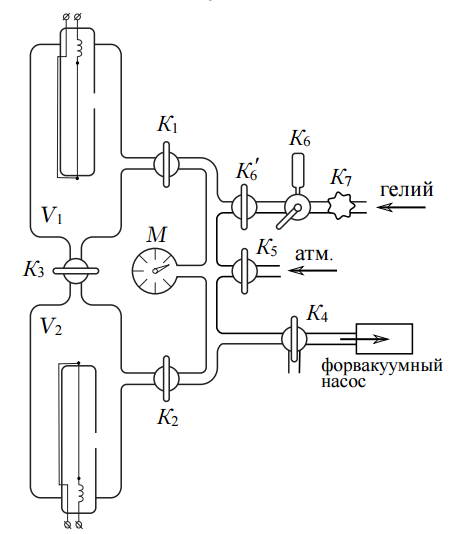
\includegraphics[width=7.5 cm]{facility.PNG}
    \caption{Установка для исследования взаимной диффузии газов}
    \label{fig:vac}
\end{figure}

\item Для измерения разности концентраций газов используется мостовая схема, представленная на рисунке 2. \\
Здесь $D_1, D_2$ - датчики теплопроводности, расположенные в сосудах $V_1$ и $V_2$. Сопротивления $R_1, R_2, R$ служат для установки прибора на нуль (балансировка моста). В одну из диагоналей моста включен гальванометр, к другой подключается небольшое постоянное напряжение. Сопротивления $R_1$ и $R_2$ спарены (их подвижные контакты находятся на общей оси) и изменяются одновременно при повороте ручки грубой регулировки. Точная балансировка выполняется потенциометром R. Балансировку необходимо проводить перед каждым экспериментом заново: при этом установка заполняется чистым газом (воздухом без гелия) при давлении, близком «рабочему» (при котором затем будут проводится измерения).

 Мост балансируется при заполнении сосудов (и датчиков) одной и той же смесью. При заполнении сосудов смесями различного состава возникает «разбаланc» моста. При незначительном различии в составах смесей показания гальванометра, подсоединённого к диагонали моста, будут пропорциональны разности концентраций примеси: $U \propto \triangle \kappa \propto \triangle n$
 
\begin{figure}[h]
    \centering
    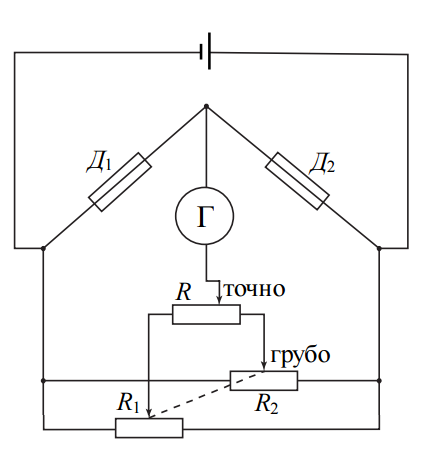
\includegraphics[width=5.5 cm]{scheme.PNG}
    \caption{Мостовая схема с датчиками теплопроводности для измерения разности концентраций газов}
    \label{fig:vac}
\end{figure} 

\item Гелий содержится в баллоне (не изображен на рис. 1) под давлением, превышающим атмосферное. Для предотвращения избыточного расхода гелия и
его неконтролируемого проникания в установку предусмотрен металлический кран (К7), отделяющий её от баллона с гелием. Его открывают только на
время непосредственного заполнения установки гелием, остальное время он должен быть закрыт. Для подачи малых порций гелия предусмотрен двухходовый кран с дозатором (рис. 4). При повороте рычажка Р в положение I гелий в небольшом количестве поступает в дозатор (если открыт К7), а при повороте Р в положение II порция из дозатора поступает в установку.

\begin{figure}[h]
    \centering
    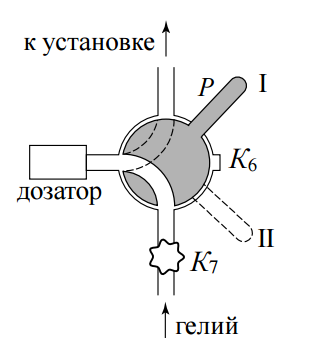
\includegraphics[width=5.5 cm]{crane.PNG}
    \caption{Кран $K_6$}
    \label{fig:vac}
\end{figure} 

\end{enumerate}

\section {Выполнение работы}

\begin{enumerate}
\item Изучим схему установки и инструкции по откачке воздуха, напуске гелия и откачке воздуха для конкретной установки. Ознакомимся с расчётной программой, используемой для считывания данных с датчиков теплопроводности. 
\item Включим питание датчиков теплопроводности и измерительного моста. Убедимся, что краны подачи гелия $K_7, K'_6$ плотно закрыты. Откачаем установку до давления $\sim 0,1$ Торр. Для этого
\begin{itemize}
\item закроем краны $K_4, K_5, K'_6$;
\item включим насос тумблером (расположен на насосе) и дадим ему откачать собственный объём ($\sim $3–5 с);
\item откроем кран $K_4$, соединив с его помощью насос и установку;
\item спустя 3-5 минут остановим откачку: отделим насос от установки краном $K_4$;
\item выключим насос тумблером (насос снабжен встроенным обратным клапаном, препятствующим выбросу масла после остановки, поэтому соединять насос с атмосферой необходимости нет)
\end{itemize}

\item Сбалансируем измерительный мост при предполагаемом «рабочем»
давлении (суммарном давлении смеси в эксперименте). В качестве на-
чального рабочего давления возьмите $P_\Sigma \sim$ 40 торр. Для этого
\begin{itemize}
\item подадим воздух краном $K_5$ непосредственно из атмосферы
\item изолируем рабочие объёмы кранами $K_1, K_2$ ($K_3$ открыт)
\item сбалансируем измерительный мост так, чтобы показания вольтметра флуктуировали в среднем около нулевого значения. Используем последовательно ручки регулировки «грубо», затем «точно». По достижении баланса переключатели моста установим на максимум. Диапазон измерений гальванометра переведём на 10мкА После балансировки и до окончания измерений при данном $P_\Sigma$ положения ручек регулировки не меняются
\end{itemize}
\item Заполним установку рабочей смесью: в сосуде $V_1$ находится воздух, а в сосуде $V_2$ - смесь воздуха с гелием. Давление должно быть одинаковым и равным рабочему давлению $P_\Sigma$. Заполнение производится в следующем порядке:
\begin{itemize}
\item откачаем всю установку до $\sim$ 0,1 Торр
\item изолируем объём $V_1$, закрыв краны $K_1$ и $K_3$ (туда не должен попасть гелий!). После этого остановим откачку
\item напустим в установку гелий до давления $P_H_e = 0,1 P_\Sigma$. Избыточное количество гелия при необходимости откачаем насосом. После этого изолируйте объём $V_2$ (краном $K_2$).
\item перекроем подачу гелия (кран $K_7$) и откачаем гелий из всех патрубков. После чего остановим откачку.
\item присоединим объём $V_1$ к установке (кран $K_1$) и заполним всю установку, исключая объём $V_2$, воздухом (без гелия) до несколько избыточного по сравнению с рабочим давления ($\sim 1,5 P_\Sigma $ в зависимости от соотношения объёмов патрубков и сосудов.
\item уравняем давление в сосудах $V_1$ и $V_2$, направив поток воздуха с избыточным давлением в сосуд с гелием. Для этого откроем кран $K_2$
при уже открытом $K_1$ (кран $K_3$ всё ещё закрыт!) Поскольку газ при адиабатическом расширении остывает, необходимо держать краны $K_1$ и $K_2$ открытыми в течение некоторого времени (30–60 с), чтобы дать давлениям выравняться при одинаковых температурах. Это время не должно быть слишком велико, чтобы диффузия гелия по патрубкам не привела к искажению приготовленного состояния.
\item запишем точное значение установившегося рабочего давления $P_\Sigma$. Изолируем объёмы $V_1$ и $V_2$, перекрыв краны $K_1$ и $K_2$. Система должна быть готова к измерениям.
\end{itemize}
\item Процесс диффузии начнётся после открывания крана $K_3$ . Приготовим компьютерную программу по дополнительному описанию. Откроем $K_3$ и измерим, как меняются показания вольтметра с течением времени U (t). Измерение будем продолжать до тех пор, пока напряжение не упадет хотя бы на 30–50\%
\item  Повторим измерения пп. 2–6 при различных значениях рабочего давления в диапазоне 40–300 торр. Результаты измерений, снятые с компьтера, занесём в таблицу 1

\item Построим графики зависимостей непосредственно изменений показания вольметра от времени. Чётко прослеживается экспоненциальная зависимость, что предсказывается теорией
\begin{figure}[h]
    \centering
    \begin{center}
    \caption{Зависимость показаний вольтметра от времени при разных значениях давления}
    \end{center}
    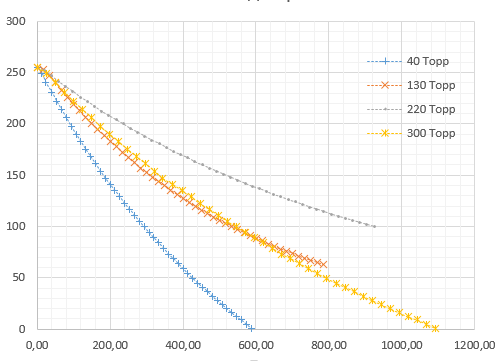
\includegraphics[width=\textwidth]{exp.PNG}
    \label{fig:vac}
\end{figure} 

\begin{figure}[h]
    \centering
    \begin{center}
    \caption{Зависимость натурального логарифма показаний вольтметра от времени при разных значениях давления (все значения)}
    \end{center}
    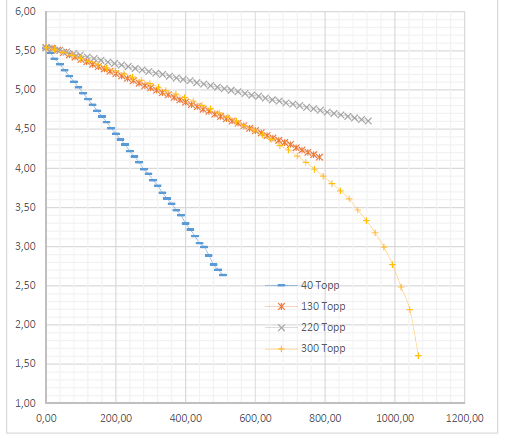
\includegraphics[width= 10 cm]{all.PNG}
    \label{fig:vac}
\end{figure} 

\begin{figure}[H]
    \centering
    \begin{center}
    \caption{Зависимость натурального логарифма показаний вольтметра от времени при разных значениях давления (без значений при 300 Торр)}
    \end{center}
    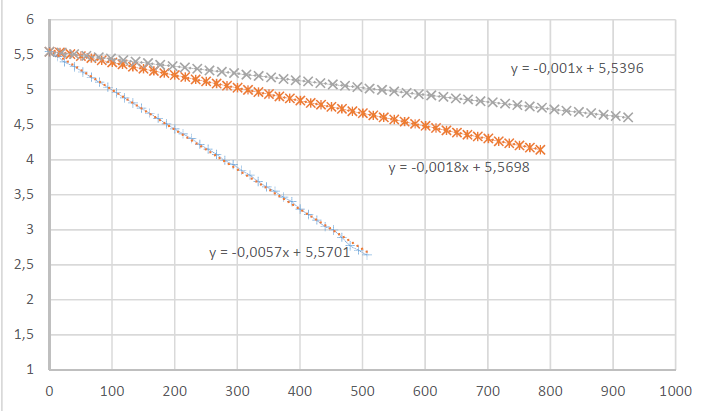
\includegraphics[width=10 cm]{notall.PNG}
    \label{fig:vac}
\end{figure} 
\item Построим графики зависисмотей показаний вольтметра т времени в логарифмическом масштабе. Теория предсказывает, что характер зависимости - обратная пропорциональность, модуль углового коэффициента уменьшается с повышением давления. Однако мы видим, что при давлении 300 Торр зависимость явно не соблюдается. Поэтому при дальнейших расчётах мы не будем учитывать этот эксперимент



\item Погрешность измерения коэффициента диффузии определим по методу наименьших квадратов:
\begin{center}
$\sigma_k = \frac{1}{\sqrt{n}}\sqrt{\frac{<ln U^2>-<ln U>^2}{<t^2>-<t>^2}-k^2}$
\end{center}

Коэффициент диффузии рассчитывается по формуле $D = -\frac{kVL}{2S}$, его ошибка будет составлять $\sigma_D = D\sqrt{(\frac{\sigma_V}{V})^2+(\frac{\sigma_k}{k})^2+(\frac{\sigma_L/S}{L/S})^2}$

Параметры установки: $V = 360 \pm 0,5 cm^3$, $L/S = (7,0 \pm 0,5) 1/cm$

\begin{center}
$\sigma_D_1 = 14\%,    D_1 = 7,56 \pm 1,06 cm^2/c$
$\sigma_D_2 = 11,2\%,     D_2 = 2,268 \pm 0,25 cm^2/c$
$\sigma_D_3 = 9,8\%,     D_3 = 1,26 \pm 0,12 cm^2/c$
$\sigma_D_4 = 26\%,    D_4 = 2,142 \pm 0,56 cm^2/c$
\end{center}

\item Построим графики зависимости коэффициента диффузии от величины, обратной давлению, по двум сериям значений: рассчитанным экспериментально и определённым с помощью компьютера, отметим пределы погрешностей. Видно, что если не учитывать точку при 300 Торр, прослеживается обратная зависимость коэффициента диффузии от давления
\begin{figure}[H]
    \centering
    \begin{center}
    \caption{Зависимость коэффициента диффузии от величины, обратной давлени. (без значения при 300 Торр)}
    \end{center}
    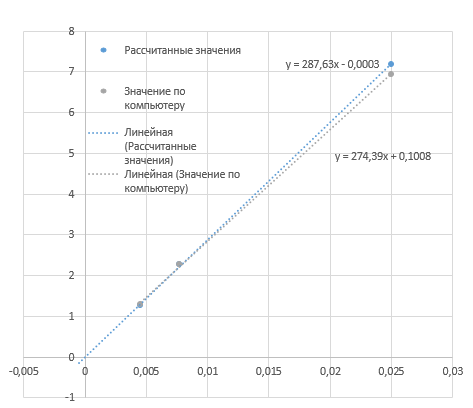
\includegraphics[width=10 cm]{atm.PNG}
    \label{fig:vac}
\end{figure} 

Экстраполируя прямую значений, полученную нами, определим коэффициент диффузии гелия в воздухе при атмосферном давлении (760 Торр). Также определим это значение, проведя прямую с учётом погрешности, и по значениям, полученным компьютером\\
\begin{center}
$D_a_1 = 0.361 cm^2/c$ - значения по компьютеру\\
$D_a_2 = 0.378 cm^2/c$ - значения по расчётам\\
$D_a_3 = 0.454 cm^2/c$ - значения по расчётам с учётом максимальной возможной погрешности\\
\end{center}

Сравним полученные значения с табличными. При температуре 273 К значение коэффициента диффузии примеси гелия в воздухе составляет $0.66 cm^2/c$. Максимально приближенное к этому значение при расчётах с учётом максимальной возможной погрешности. Значения по компьютеру, по расчётам и по теории совпали по порядку величины, но не совпадают в пределах допустимой погрешности. 

\item Оценим длину свободного пробега молекулы по формуле 
\begin{center}
$\lambda = \frac{3D}{\bar v} \sqrt{\frac{\pi \mu }{8RT}} = 235.3 $ нм
\end{center}
При нормальных условиях табличное значение для длины свободного пробега молекулы гелия равно 180 нм. Экспериментальное и теоретическое значения совпали по порядку величины.

Наконец, оценим эффективное сечение столконевний атомов гелия с частицами воздуха при температуре 299 К и давлении $10^5$ Па:

\begin{center}
$\sigma = \frac{1}{\lambda n}$\\
$\sigma = \frac{kT}{\lamda P} = 1.6 * 10^-^1^7$ м
\end{center}

\end{enumerate}
\newpage

\section{Вывод}
В ходе работы было экспериментально определено значение коэффициента диффузии для примеси гелия в воздухе. Был проведён эксперимент, при котором измерялась зависимость показаний вольтметра, соединённого с датчиком, определяющим разность концентраций примеси и основного газа. Полученные значения зависимости коэффициента диффузии от давления были экстраполированы к прямой и экспериментаьно было получено значение коэффициента диффузии при атмосферном давлении. Определённое значение $D_a = 0.378 cm^2/c$  по порядку величины совпало с табличным $D_a_t = 0.66 cm^2/c$. Также были оценены длина свободного пробега молекулы гелия при нормальных условиях ($\lambda =  235.3$ м) и эффективное сечение столконевний атомов гелия с частицами воздуха при температуре 299 К и давлении $10^5$ Па ($\sigma = 1.6 * 10^-^1^7$ м).\par
Причины расхождения теории и эксперимента не могут быть точно описаны. Температура, при которой проводился эксперимент, была равна 299 К, табличные значения определены для температуры 273 К, причём при более высокой температуре значения оказались ниже, хотя теория предсказывает обратную зависимость: уравнение Эйнштейна для связи коэффициента диффузии и подвижности частицы: $D = kTB$, подвижность частицы также прямо пропорциональна значению температуры. Теоретически, с повышением температуры коэффициент диффузии должен повыситься, но он наоборот оказался ниже. \par
В эксперименте был один существенный недостаток: измерения проводились при большой разности начального и конечного давлений (от 40 до 300 Торр с шагом в 90 Торр). Повышение полученного нами значения коэффициента диффузии при 300 Торр не удалось описать теоретически. У студентов, проводивших эксперимент с шагом около 20 Торр, экстраполированная прямая (рис. 7) не содержала "выпадающего"  значения. Возможно, если бы эксперимент проводился с учётом этих замечаний, результат оказался бы более приближенным к теоретическому значению

\end{document}
